\documentclass[11pt, a4paper]{article}

\usepackage[margin=1in]{geometry} % manage page dimentions
\usepackage[utf8]{inputenc} % utf-8 encoding
\usepackage[italian]{babel} % italian default text
\usepackage[hidelinks]{hyperref} % link references
\usepackage{bookmark} % 
\usepackage{import} % import other .tex files
\usepackage{amsmath} % math commands
\usepackage{amssymb} % math symbols
\usepackage{amsthm} % math environments
\usepackage{amsmath} % equation align
\usepackage{siunitx} % SI unit
\usepackage{booktabs} % tabular enhance
\usepackage{multirow} % dinamic tabular cell dimentions
\usepackage{longtable} % multi-page table
\usepackage[labelfont=bf, skip=.5em, font=small]{caption} % beautiful caption
\usepackage{subcaption} % subfigure
\usepackage{graphicx} % import graphics
\usepackage{fancyhdr} % custom page header and footer

% \showthe\textwidth

\graphicspath{{../assets/}} % base graphics path

\setlength{\parskip}{1em} % distance between paragraphs
\setlength{\parindent}{0em} % indentation at beginning of paragraph
\setlength{\headheight}{13.59999pt}

\numberwithin{equation}{section} % equation tag relative to section

\pagestyle{fancy}
\fancyhead[L]{\nouppercase{\leftmark}}
\fancyhead[R]{\textbf{Pag. \thepage}}
\fancyfoot{}

\title{Esperienza 3}
\date{9/12/2021}
\author{}

\begin{document}

\maketitle

\thispagestyle{empty}

\tableofcontents

\section{Obiettivo dell'esperienza}

Lo scopo dell'esperienza è quello di calcolare il valore della resistenza e della capacità di un circuito RC. Per farlo si analizza come varia la differenza di potenziale ai capi di R (\autoref{fig:circuito R}) e/o ai capi di C (\autoref{fig:circuito C}) quando si sottoposto il circuito ad una tensione variabile.

\begin{figure}[ht!]
    \centering
    \begin{subfigure}[c]{.3\textwidth}
        % \import{../assets/}{circuito_osc_R.pdf_tex}
        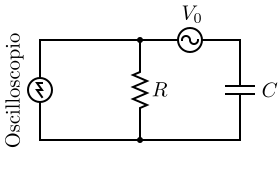
\includegraphics[width=\textwidth]{circuito_osc_R.pdf}
        \caption{Misure ai capi di R}
        \label{fig:circuito R}
    \end{subfigure}
    \hspace{1in}
    \begin{subfigure}[c]{.3\textwidth}
        % \import{../assets/}{circuito_osc_C.pdf_tex}
        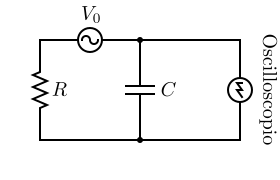
\includegraphics[width=\textwidth]{circuito_osc_C.pdf}
        \caption{Misure ai capi di C}
        \label{fig:circuito C}
    \end{subfigure}
    \caption{Schema circuito}
  \end{figure}

\section{Strumenti e materiali}

\begin{itemize}
    \item Generatore di tensione AC
    \item Multimetro digitale (utilizzato come ohmetro)
    \item Oscilloscopio
    \item Cavi
    \item Breadboard
    \item Resistore
    \item Condensatore
\end{itemize}

\section{Onda quadra}

La prima parte dell'esperimento consiste nell'applicare ai capi del circuito una tensione variabile secondo un'onda quadra di ampiezza \(V_{0}\). La frequenda dell'onda è stata scelta in modo da permettere al condensatore di completare il regime transitorio, passando da una tensione \(V_{0}/2\) fino ad una tensione \(- V_{0}/2\). La curva osservata nell'oscilloscopio rappresenta la tensione \(V_{C}\) ai capi del condensatore in funzione del tempo \(t\) e segue l'\autoref{eq:regime transitorio onda quadra}.

\begin{equation} \label{eq:regime transitorio onda quadra}
    V_{C} = V_{0} \cdot e^{-t/RC} - V_{0}/2
\end{equation}

Per prendere le misure il sistema di riferimento è stato traslato in modo da porre come \(0\) delle ordinate il valore \(- V_{0}/2\) e ottenere l'\autoref{eq:regime transitorio condensatore}.

\begin{equation} \label{eq:regime transitorio condensatore}
    V = V_{0} \cdot e^{-t/RC}
\end{equation}

Noto il valore di \(R = (1.874 \pm 0.004) \; \unit{k\Omega}\), misurato tramite il multimetro, si vuole ottenere il valore di \(C\).

\subsection{Dati ed errori}

Attraverso l'oscilloscopio si è fissato il primo cursore in corrispondenza dell'asintoto della curva a \(- V_{0}/2\), questo sarà lo \(0\) delle ordinale, il secondo cursore è stato fatto variare in modo da ottenere la differenza di potenziale al variere del tempo. Le misure ottenute sono riportate, insieme ai loro errori già arrotondati, nella \autoref{tab:misure onda quadra}.

% Attraverso l'oscilloscopio, con l'ausilio dei cursori, è stata misurata la differenza di potenziale ai capi del condensatore al variare del tempo.

\begin{table}[ht!]
    \centering
    \caption{Misure dell'onda quadra}
    \import{../tables/}{onda_quadra_Vt.tex}
    \label{tab:misure onda quadra}
\end{table}

\subsection{Analisi dati}

\begin{equation*}
    V = V_{0} \cdot e^{-t/RC} \implies \ln(V) = \ln(V_{0} \cdot e^{-t/RC}) = \ln(V_{0}) - \frac{t}{RC}
\end{equation*}

Quindi riportando le misure in un grafico semi-logaritmico, come fatto in \autoref{fig:onda quadra pendenze}, ci si aspetta di ottenere una funzione lineare

\begin{figure}[ht!]
    \includegraphics{onda_quadra_V(t)_pendenze.pdf}
    \caption{Grafico semi-logaritmico misure dell'onda quadra}
    \label{fig:onda quadra pendenze}
\end{figure}

La retta di massima pendenza passa per i punti \((-0.2, 7)\) e \((35, 0.6)\) mentre la retta di minima pendenza passa per i punti \((0.2, 7)\) e \((34, 0.5)\)

\begin{equation*}
    m_{max} = \frac{\ln(7/0.6)}{- 0.2 - 35} = - 0.06979
    \qquad
    m_{min} = \frac{\ln(7/0.5)}{0.2 - 34} = - 0.07808
\end{equation*}

\begin{align*}
    m_{best} &= \frac{m_{max} + m_{min}}{2} = - 0.0739 \approx - 0.074 \\
    \delta m &= \frac{m_{max} - m_{min}}{2} = 0.0041 \approx 0.004
\end{align*}

\begin{equation}
    m = - 0.074 \pm 0.004
\end{equation}

Essendo \(m = \dfrac{1}{RC}\) e conoscendo il valore di \(R = (1.874 \pm 0.004) \; \unit{k\Omega}\).

\begin{align*}
    \varepsilon_R &= \frac{0.004}{1.874} = 0.0021 \approx 0.002 \\
    \varepsilon_m &= \frac{0.004}{0.074} = 0.054 \approx 0.05 \\
    \varepsilon_C &= \sqrt{\varepsilon_R^{2} + \varepsilon_m^{2}} = 0.050 % review
\end{align*}

\begin{equation}
    C = \frac{R}{m} = 25.32 \pm 1.27 \approx (25.3 \pm 1.3) \; \unit{nF}
\end{equation}

\section{Onda sinusoidale}

\subsection{Dati ed errori}

\subsection{Analisi dati}

\section{Conclusioni}

\end{document}